\subsection{Long-baseline neutrino beams }

Neutrino beams~\cite{Kopp2007101} based on particle accelerators have been used since the 1960s, when they provided the evidence for the existence of two types of neutrino, $\nu_e$ and $\nu_\mu$. The general design is based on a high intensity proton beam impinging on a target and producing pions and kaons through interactions on the target nuclei. 
These mesons decay in a dedicated volume downstream of the target, creating mainly a $\nu_\mu$ beam.  

The long baseline beams are based on the so called wide band beam concept. Here the secondary charged mesons are focused using a system of magnetic devices, called horns. The horns, usually with a cylindrical symmetry around the beam, are pulsed with a very intense current in coincidence with the arrival of the beam. 
%The ratio between the primary proton energy and the typical neutrino energy is %at least a factor ten, and the neutrino spectrum extends for about a decade %around this typical energy.  

The flux is tuned in such a way that the phase $\Delta m^2_{32} L/ (4 E)$ reaches $\pi/2$ for the design baseline $L$ and the peak energy $E$, in order to probe the atmospheric oscillation sector with the beam $\nu_\mu$. To do so, the proton energy, the target length and width, the focussing system and the decay volume length and width need to be accurately designed and optimized.   

An off-axis neutrino beam \cite{1995bnl} relies on the following idea: as the $\nu_\mu$ are mainly produced by the two-body decays of pions, there is a correlation between pion energy $E_\pi$, the neutrino energy $E_\nu$ and the decay angle $\theta$ 
\begin{equation}
E_\nu = \frac{(1-(m_\mu/m_\pi)^2) E_\pi}{(1+\gamma^2 \theta^2) } 
\end{equation}
valid in the limit of small angles.

Neutrinos emitted at a small angle with respect to the pion direction have a distinct narrow spectrum peaking at a much lower energy with respect to the on axis beam. This feature that has been used by the T2K and \nova experiments, offers several advantages because it avoids the large high energy tail of the on axis beam, thereby reducing some background reactions. 

\begin{figure}[htbp]
\centering
%\includegraphics[width=0.5\linewidth]{energy_miniboone.eps}
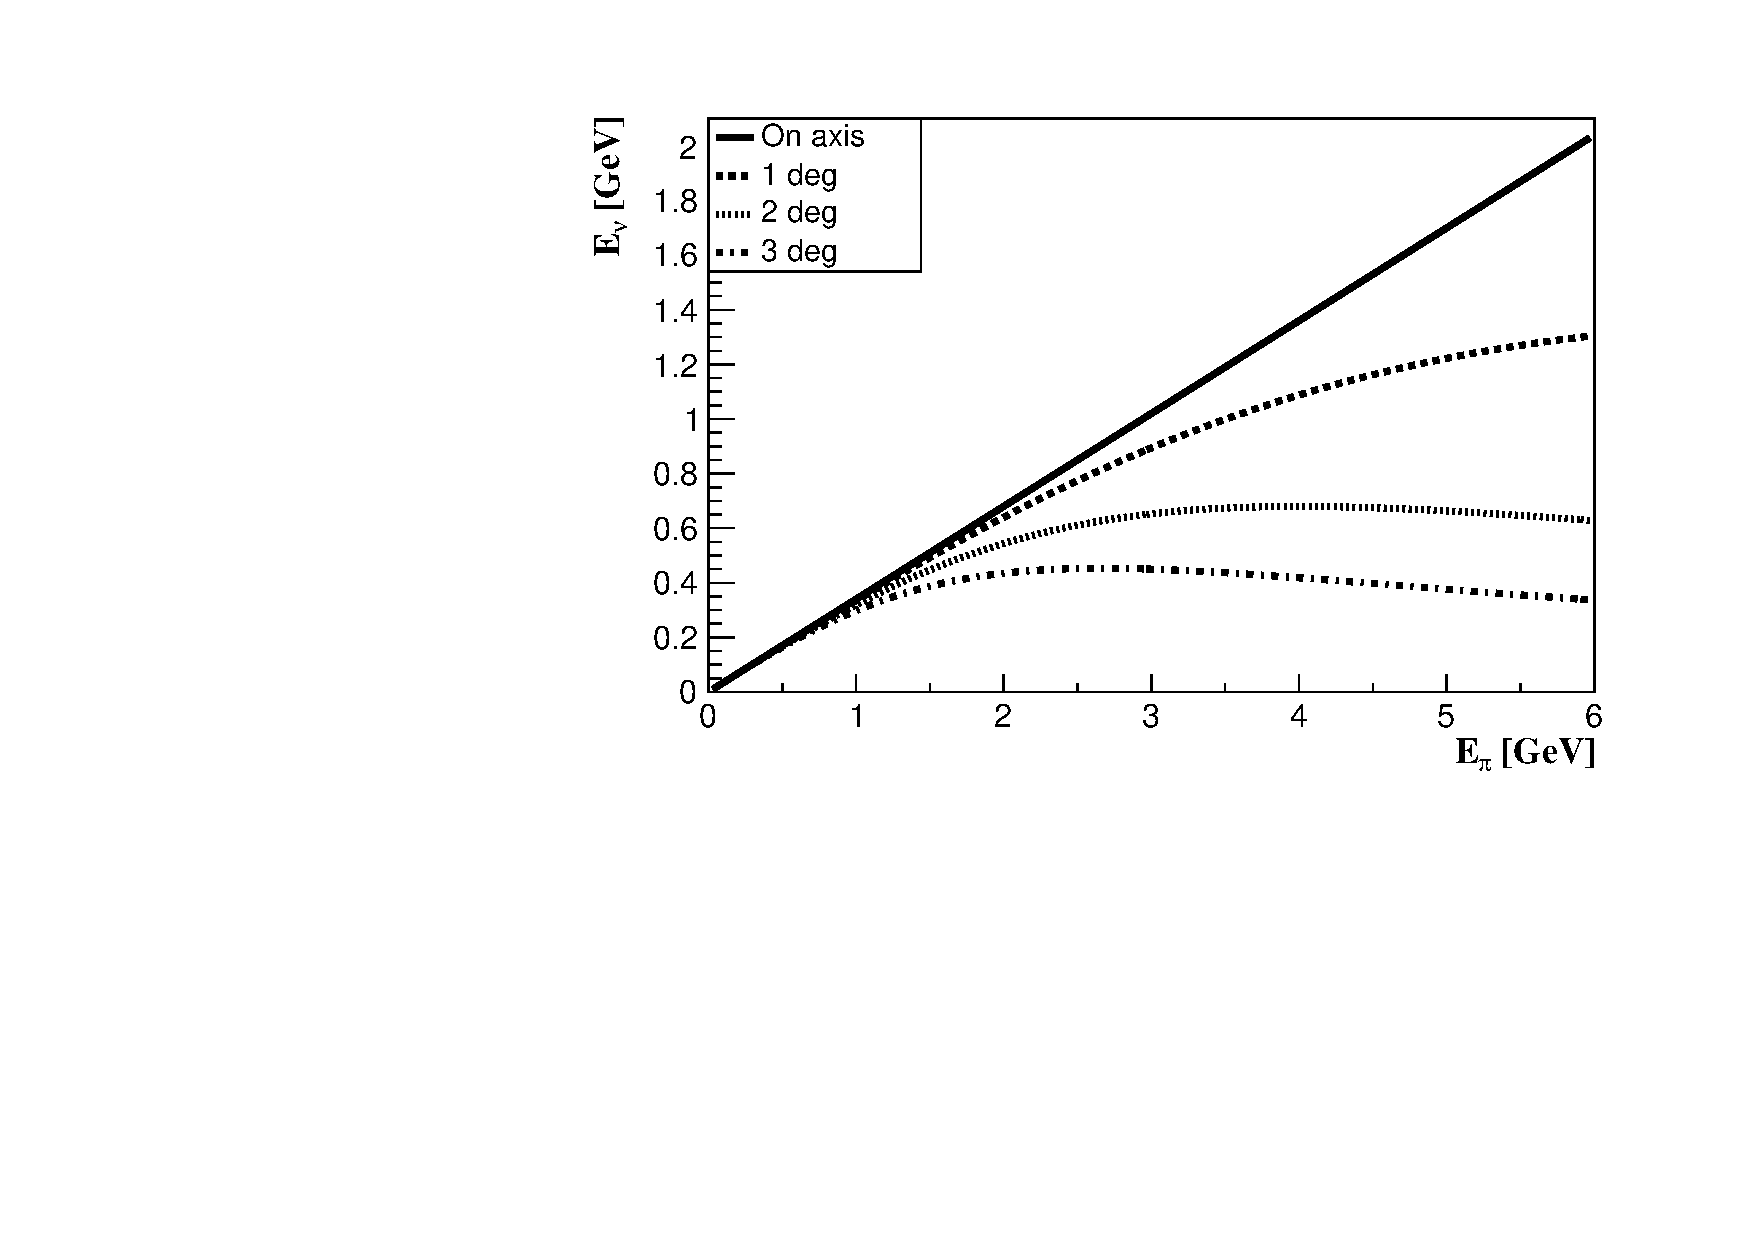
\includegraphics[width=0.6\linewidth]{figures/offaxis.pdf}
  \caption{Neutrino energy as a function of the pion energy for on-axis decays and several off-axis angles. For a non-zero off-axis angle, the neutrino energy reaches a maximum. This feature is currently exploited in the T2K and \nova experiments.}
 \label{fig:offaxis}
 \end{figure}


As the neutrino beam is a tertiary beam, it is necessary to include in the experimental apparatus monitoring devices to ensure that it is stable in intensity and direction. To this effect, muon detectors, sensitive to the muons produced by the pion decays, are placed close to the end of the decay volume. Moreover, as the neutrino flux and cross-sections and the beam composition are not known with sufficient precision, a near detector is located close to the target station (typically within a few hundred meters). The near detector constrains the neutrino interaction rate, proportional to the product t=of neutrino flux and the cross-section. Moreover, the near detector allows to measure the beam composition and to perform study of several neutrino cross-section.    

Description of T2K beam line if space allows.

\begin{table}
\centering
\begin{tabular}{|c|c|c|c|c|c|}
  \hline
  Exp. & Energy (GeV) & Power (kW) & L (km) & FD mass (kt) & POT \\ 
  \hline
K2K & 30 & & 250 & 22.5 & \\
MINOS & 120 & 700 & 790 & 5.4 &\\
OPERA & 450 & 732 &  & & 1.8 10$^{20}$\\
T2K & 30 & 750 & 295 & 22.5 & 8 10$^{21}$\\
\nova & 120 & 700& 810 & 14 & \\
HK & 30 & & & & \\
DUNE & 120 & 1200 & 1300 & 40 &\\
  \hline
\end{tabular}
\caption{Parameters of recent and future long baseline experiments. Energy and power refer to the primary proton beam, L is the baseline, FD the mass of the far detector. POT (Proton On Target) represents the integrated dataset as of 2016.}
\end{table}

\subsubsection{Flux and cross-section systematic uncertainties in long-baseline experiments}
\label{sec:beamsyst}
The measurement of neutrino oscillations has now entered the precision era. Particularly long-baseline neutrino oscillation experiments require a deep knowledge of the systematic uncertainties related to neutrino fluxes and neutrino cross-sections to perform measurements of oscillation parameters. 

A common strategy to reduce systematic uncertainties, used in most of the long baseline experiments, is the use of a Near Detector complex, located at few hundreds of meters from the beam target where neutrinos are detected before the oscillations. In this way the neutrino spectrum and the flavor composition of the beam can be precisely measured before the oscillations and is used to determine the expected spectra at the far detector if there were no oscillations.

Some long-baseline experiments, as for example MINOS and \nova, uses as near detector a detector that has the same composition as the far detector so that cross-section uncertainties due to the different target nuclei or detector systematic uncertainties are minimized in the extrapolation. Other experiments, as for example K2K and T2K, uses a set of near detector, with different target nuclei, in order to maximize the information on the cross-section models.

In this section, as an example, we will briefly describe how the T2K experiment uses the near detector data to reduce the systematic uncertainties in the oscillation analysis. The T2K near detector, called ND280, is magnetized, with several sub-detectors installed within the ex UA1/NOMAD magnet that provides a 0.2 T magnetic field. For the oscillation analysis the ND280 tracker system is used, comprising 2 Fine Grained Detectors (FGD) interleaved to 3 Time Projection Chambers (TPC). The FGDs act as an active target for neutrino interactions (each with a mass of $\sim1.5~ton$ (check). Particles produced in the FGD enter the TPCs where the charge and the momentum of the tracks is reconstructed as well as the particle identification based on the measurement of the energy loss in the gas. One important point to notice is that one of the two FGD is a fully active detector while in the second one scintillator layers are interleaved with inactive water layers, allowing to select neutrino interactions on carbon and on oxygen that is the same target as the far detector, SK. 
    
At T2K energies most of the \num charged current neutrino interactions produce only one track in the final state, the muon. The presence of the magnetic field allows to reconstruct the charge of the muon, distinguishing between negative muons produced by \num and positive leptons produced by \numb interactions.
In some cases neutrinos give enough energy to the target nuclei producing also pions or protons that can, in some cases, enter the TPC. 
For \num selections, ND280 distinguishes three cases: only the muon is reconstructed (CC0$\pi$), the muon and one negative pion is also reconstructed (CC1$\pi$) and the other cases in which (CCother). For \numb selections interaction with one track are separated from the interactions with more than one track.
  
The same selections are applied to interactions in both the FGD and all the samples are then fit to reduce systematic uncertainties on the flux and cross-section model. 
The main uncertainty on the flux model is due to the hadron production cross-section. Data from the NA61/SHINE experiment at CERN are used. In NA61/SHINE a proton beam is accelerated to 30 GeV/c and strikes a target. Hadrons produced are measured with a system of TPCs and Time Of Flight detectors, and double differential cross-section (in angle and momentum) are extracted. Thanks to NA61/SHINE data the uncertainties on the neutrino fluxes, prior to the ND280 fits, are reduced to the 10-15\% level.

For the cross-section model, the priors are based, as much as possible, on external experiments such as MiniBooNE and MINERvA with uncertainties large enough to allow the ND280 data to constraint those parameters. Various parameters are defined to describe the theoretical uncertainties on the different neutrino interaction channels important at T2K energies. An important aspect is that, for the first time, effects related to the multi-nucleon emissions are included in this analysis, based on the Nieves model~\cite{Nieves:2011yp}

To reduce flux and cross-section uncertainties, the ND280 samples are binned in the kinematic variables \ptheta according to the muon momentum and angle with respect to the beam direction. Data and Monte Carlo are fitted using a binned likelihood, where the prediction for each bin depends on the flux, cross-section and detector systematic parameters. 

The result of the fit is a set of point estimates and covariance for the systematic scaling factors for the unoscillated neutrino flux at SK. The impact of the ND280 fit on the total error budget in the T2K oscillation analysis is shown in Tab.~\ref{tab:t2ksyst}: a reduction of the systematic uncertainties from $\sim15\%$ to $\sim5\%$ is obtained thanks to the near detector fit.

In the case of \nova, they profit of the fact that the near and the far detector are identical and use a calorimetric approach in which all the energy observed in the event at the near detector is reconstructed and is then unfolded to obtain the expected true neutrino energy. The far to near ratio and the oscillation probabilities are then applied to obtain the expected true energy spectrum at the far detector. This method allow to reduce the total systematic uncertainty to level similar to the ones obtained by T2K.

\subsubsection{Results from long-baseline accelerator experiments K2K MINOS T2K \nova}

K2K (KEK-to-Kamioka) was the first long baseline neutrino beam, using Super-Kamiokande as its far detector at 290 km from the neutrino production. Operating between 1999 and 2004, it has measured the disappearance of $\nu_\mu$: 112 events were observed, while 158.1$^{+9.2}_{-8.6}$ were expected without oscillation, a 4.3 $\sigma$ effect~\cite{Ahn:2006zza}. This measurement has confirmed neutrino oscillation as the explanation for the atmospheric neutrino disappearance. 

Further precision measurements of the $\nu_\mu \rightarrow \nu_\mu$ were reported by MINOS, T2K and NOvA. In particular, T2K and \nova use a narrow band beam, based on the off-axis design, that is particularly suited for the measurement of \num disappearance once the mass square difference is known. For a given \dmsq and a given baseline distance, in fact, the oscillation probability depends on the neutrino energy that can be tuned by changing the off-axis angle. In the case of T2K (L=295~km) the maximum of the oscillation is at an energy of 600 \mev while in the case of \nova  (L=810~km) the maximum is at 1800 \mev. 

While the most recent analyses published by T2K do a global fits of appearance and disappearance modes to extract the maximum of the information on neutrino oscillations in the PMNS framework, disappearance analyses only have also been done by T2K in order to test the PMNS framework. In the \num disappearance probability in fact there are no CP odd terms so the disappearance probability is expected to be the same for \num and \numb. Previous results from MINOS showed some tensions between neutrinos and antineutrinos. 
Based on \nupot protons-on-target (POT) collected in neutrino mode and \nubpot POT collected in antineutrino mode, T2K has observed 135 (66) \num (\numb) candidates at SK with 522 (185) events expected in case of no-oscillations and 135.8 (64.2) events expected for maximum disappearance. The reconstructed energy spectrum for both, \num and \numb surviving events are shown in Fig.~\ref{fig:t2kdis}. Thanks to the use of the Near Detector data described in Sect.~\ref{sec:beamsyst}, the systematic uncertainties on these measurements are smaller than 5\% and a precise measurement of \thatm and \dmsq is obtained as shown in Fig.~\ref{fig:t2katm-contour}. The oscillation parameters measured are in excellent agreement between neutrinos and antineutrinos and both are compatible with maximal mixing for \thatm.

\begin{figure}[htbp]
\centering
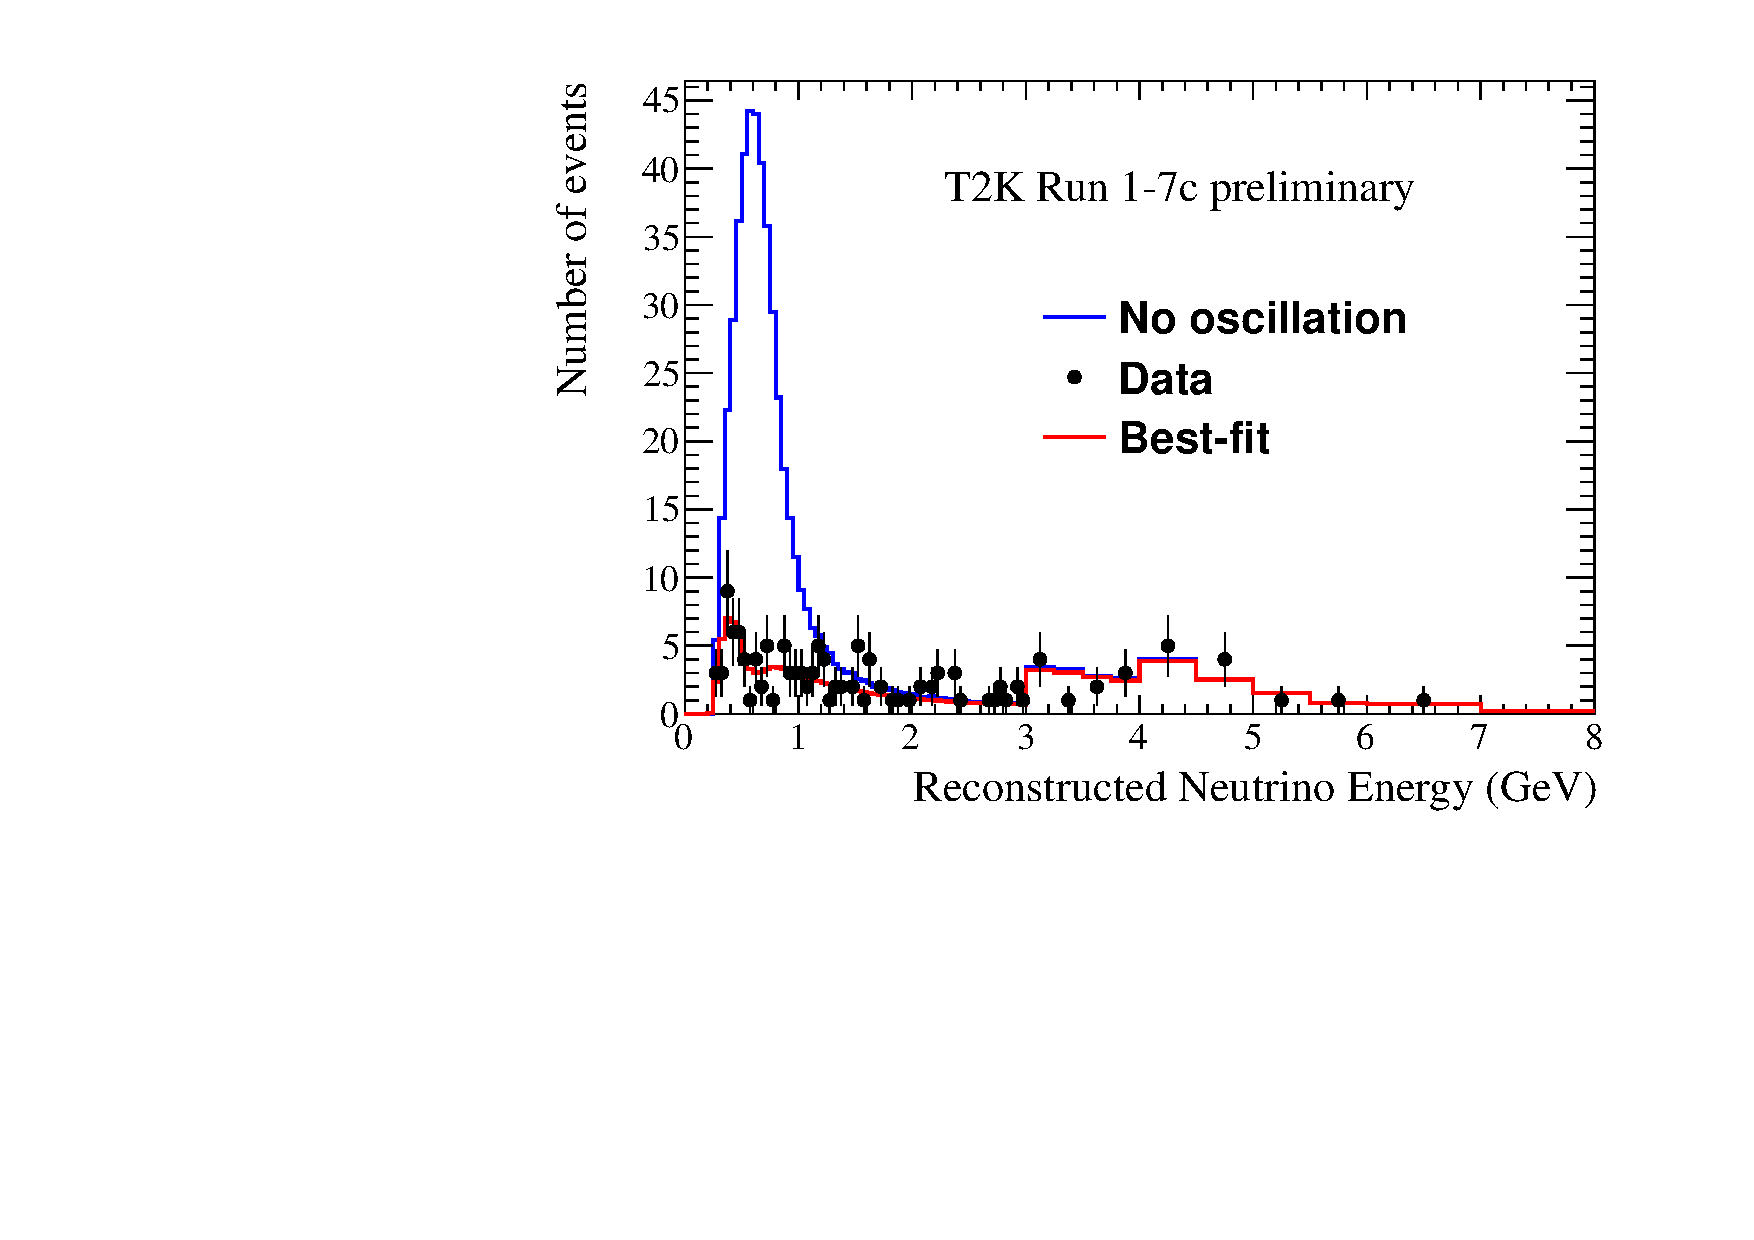
\includegraphics[width=0.3\linewidth]{figures/bestfit_sinsqth23vsdcpvsmh_1rmu_run17.pdf}
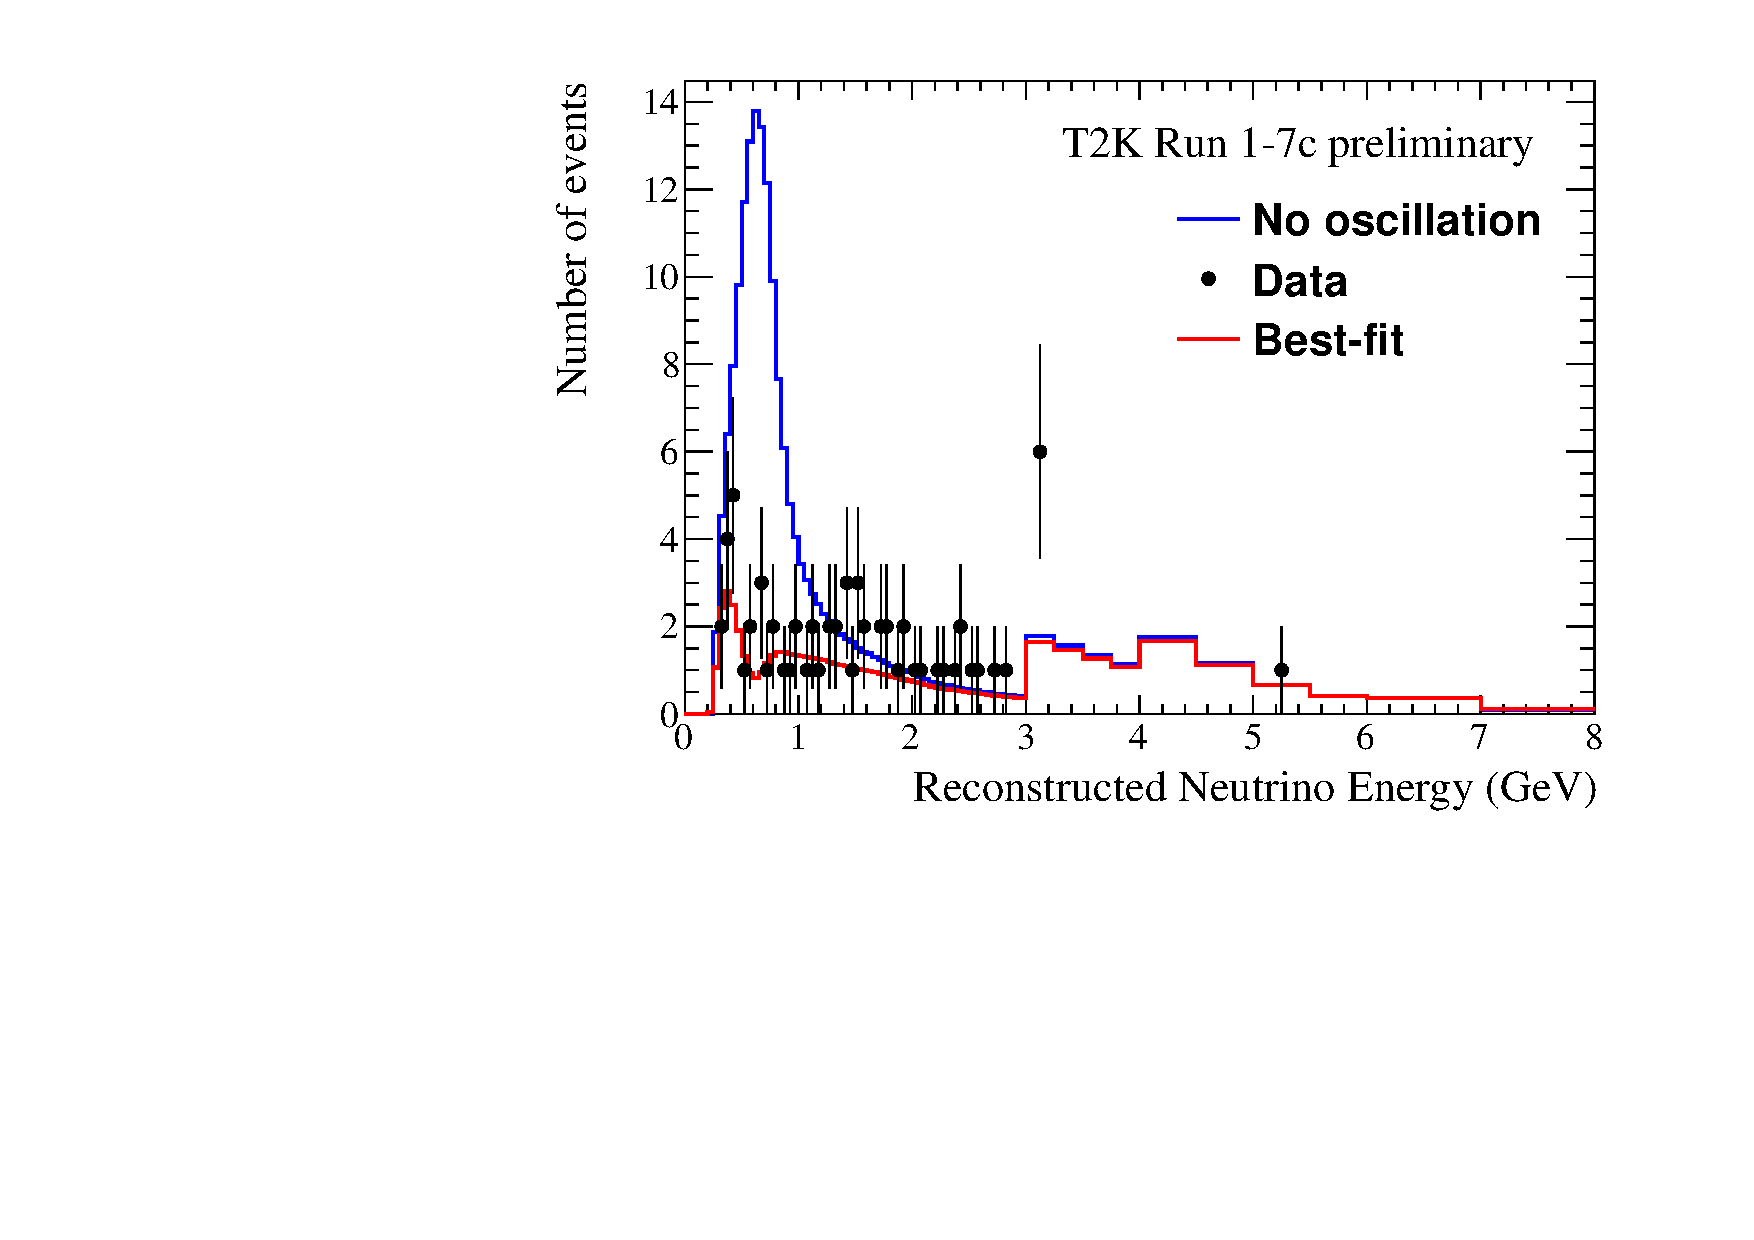
\includegraphics[width=0.3\linewidth]{figures/bestfit_sinsqth23vsdcpvsmh_rhc1rmu_run17.pdf}
  \caption{
Reconstructed \num and \numb energy spectrum by the T2K collaboration for data, best-fit prediction, and
unoscillated prediction. %Bottom: Ratio of oscillated to unoscillated events as a function of
%neutrino energy for the data and the best-fit spectrum.
}
 \label{fig:t2kdis}
 \end{figure}

\begin{figure}[htbp]
\centering
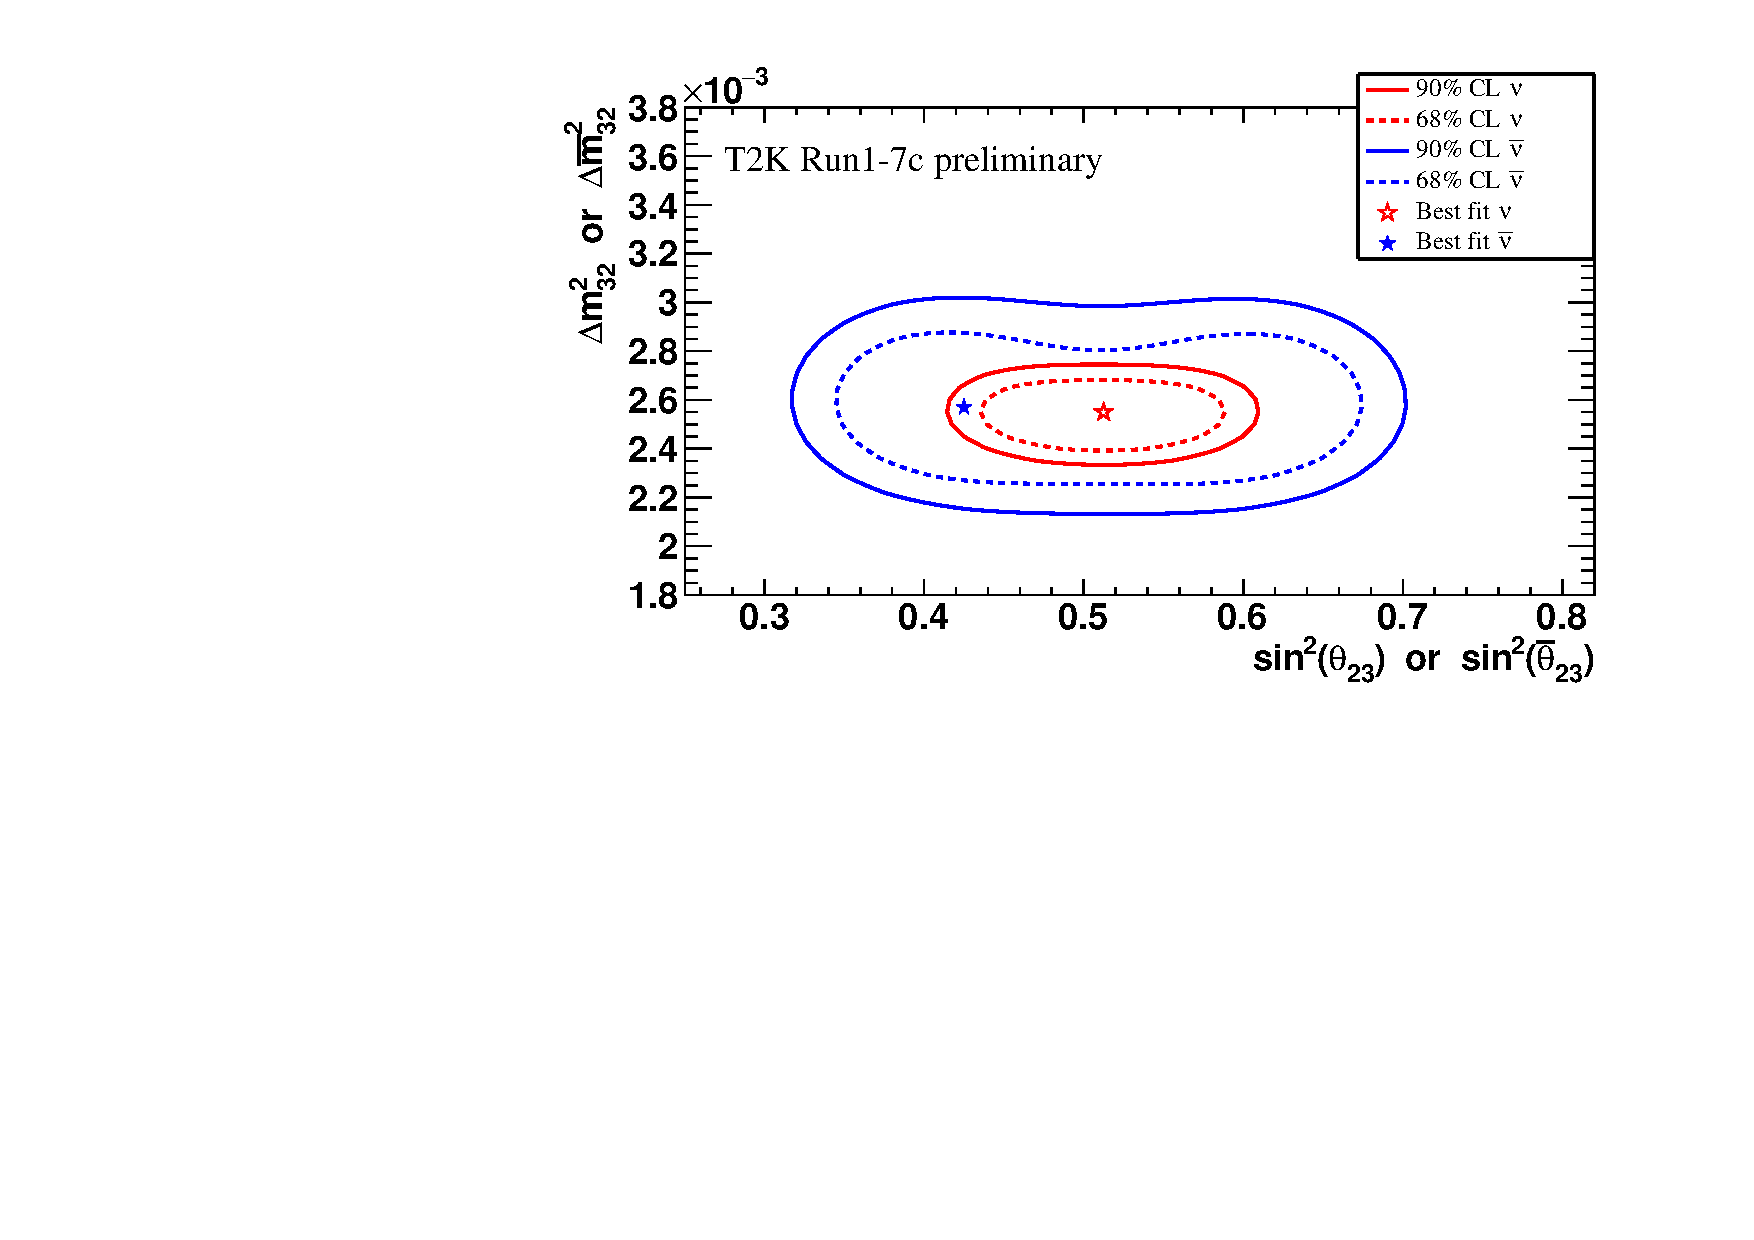
\includegraphics[width=0.6\linewidth]{figures/nu_vs_nubar_datafit_17c_nh.pdf}
  \caption{$\Delta m^2 $ versus \stt for neutrinos and antineutrinos parameters. The constant $\Delta \chi^2$ critical values in the gaussian approximation are shown.}
 \label{fig:atm-contour}
 \end{figure}

\nova has also reported a measurement of \num disappearance using \novapot POT and by selecting \mmu-like candidates at the far detector. They observed 78 events in the far detector, while $473\pm30$ were expected without oscillations. This result lead to some tensions, especially with the T2K experiment, since maximal mixing is excluded by NOvA at $2.5\sigma$ as shown in Fig.~\ref{fig:atm-contour}. 

\begin{figure}[htbp]
\centering
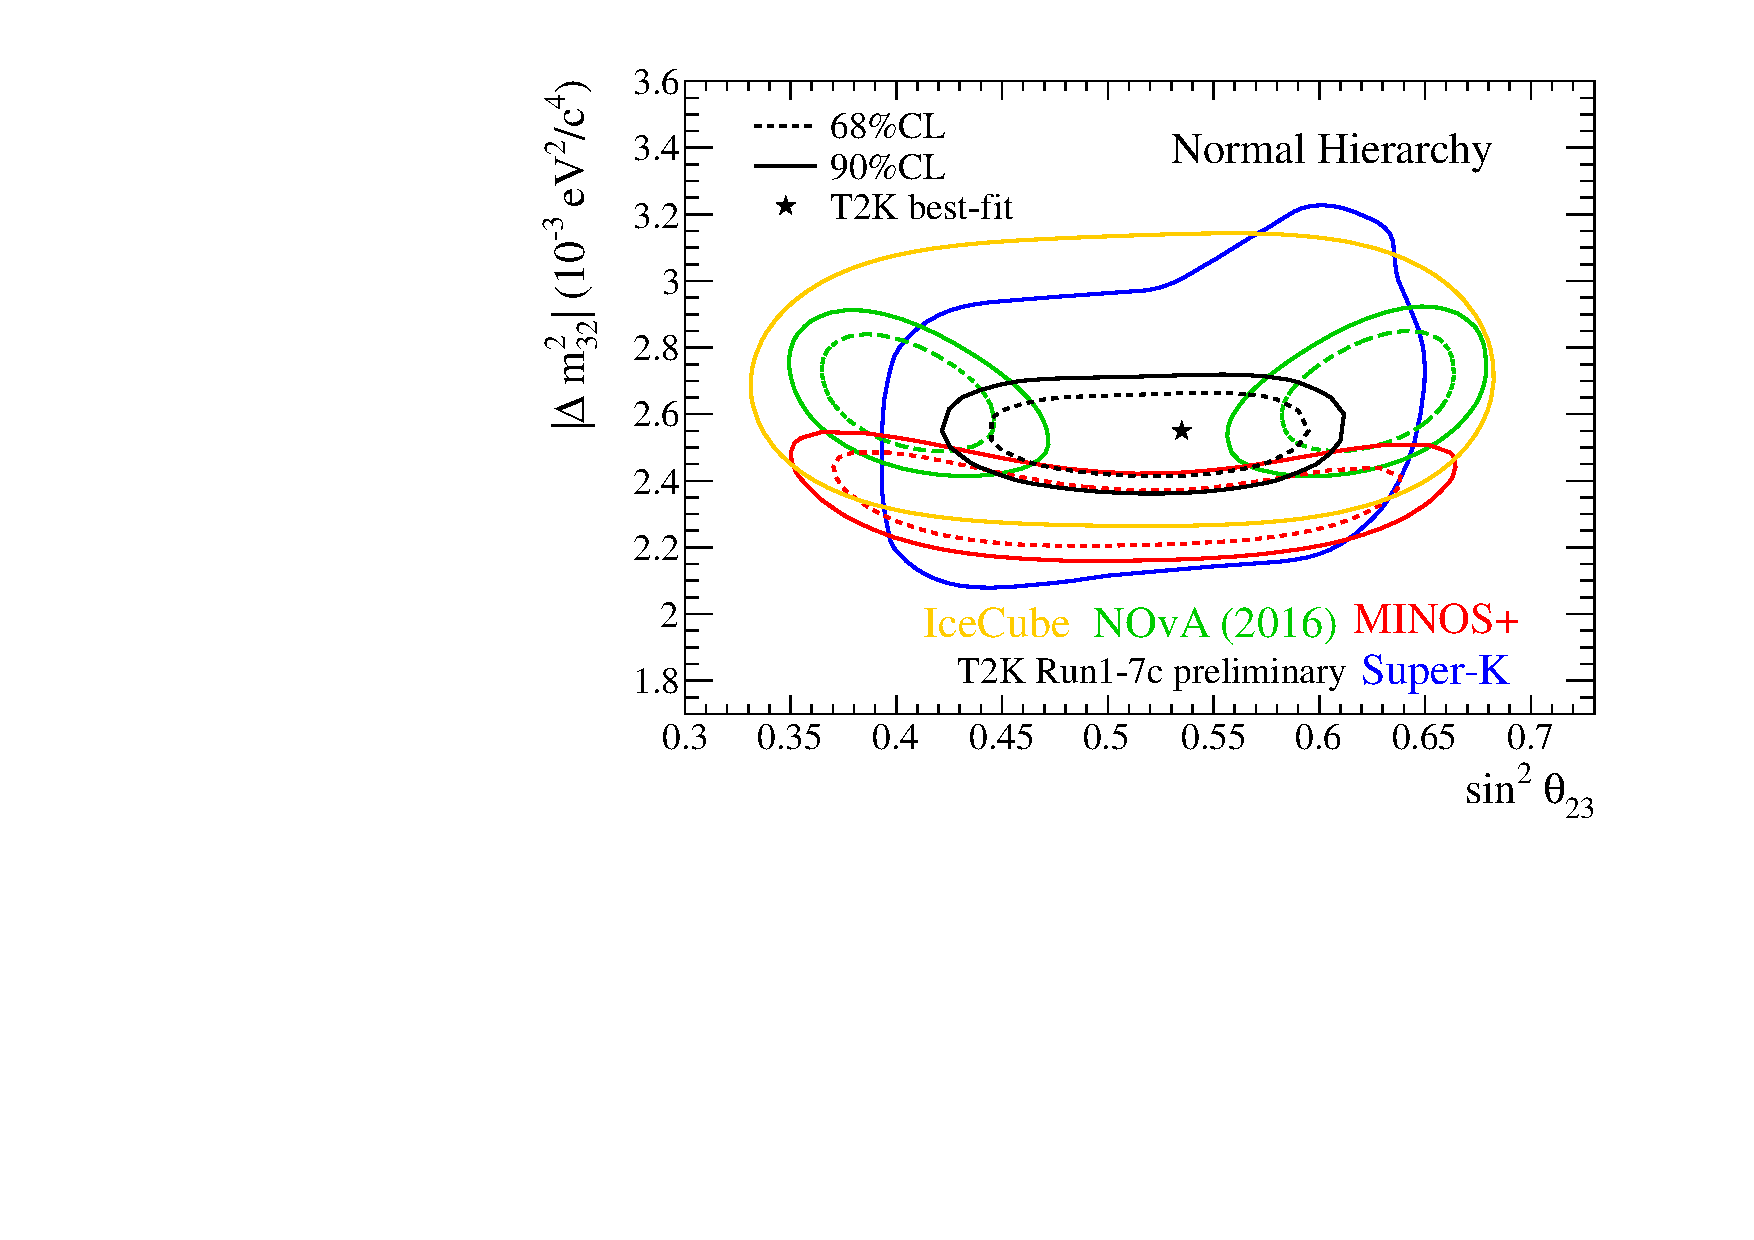
\includegraphics[width=0.5\linewidth]{figures/sinsqth23vsdmsq_react_othexp_nh.pdf}
%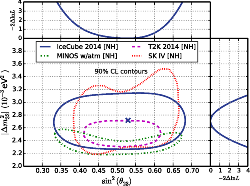
\includegraphics[width=0.6\linewidth]{figures/atm-contour.pdf}
  \caption{
Measured $\Delta \chi^2$ distributions as a function of $\sin^2 \theta_{23}$, $\Delta m^2_{32} (\Delta m^2_{13})$ for T2K, Super-K (PoS ICRC2015 (2015) 1062), Minos+ (Neutrino 2014 conference), \nova (Phys.Rev. D93 (2016) 051104, arXiv 1601.05037) and IceCube DeepCore (Phys.Rev. D91 (2015) 072004, arXiv 1410.7227).}
 \label{fig:atm-contour}
 \end{figure}
 
The two collaborations are working to understand this difference that could still be simply due to statistical fluctuations. A comparison between reconstructed energy spectrum for the best-fit and the one obtained by imposing maximal mixing in \nova is shown in Fig.~\ref{fig:novadiscomparison}. Something similar is done by T2K comparing their data, the T2K best fit and the spectrum obtained by imposing the NOvA best-fit oscillation parameters as shown in Fig.~\ref{fig:t2kdiscomparison}. Additional data from both, T2K and NOvA will help to clarify the situation. 
 
 \begin{figure}[htbp]
\centering
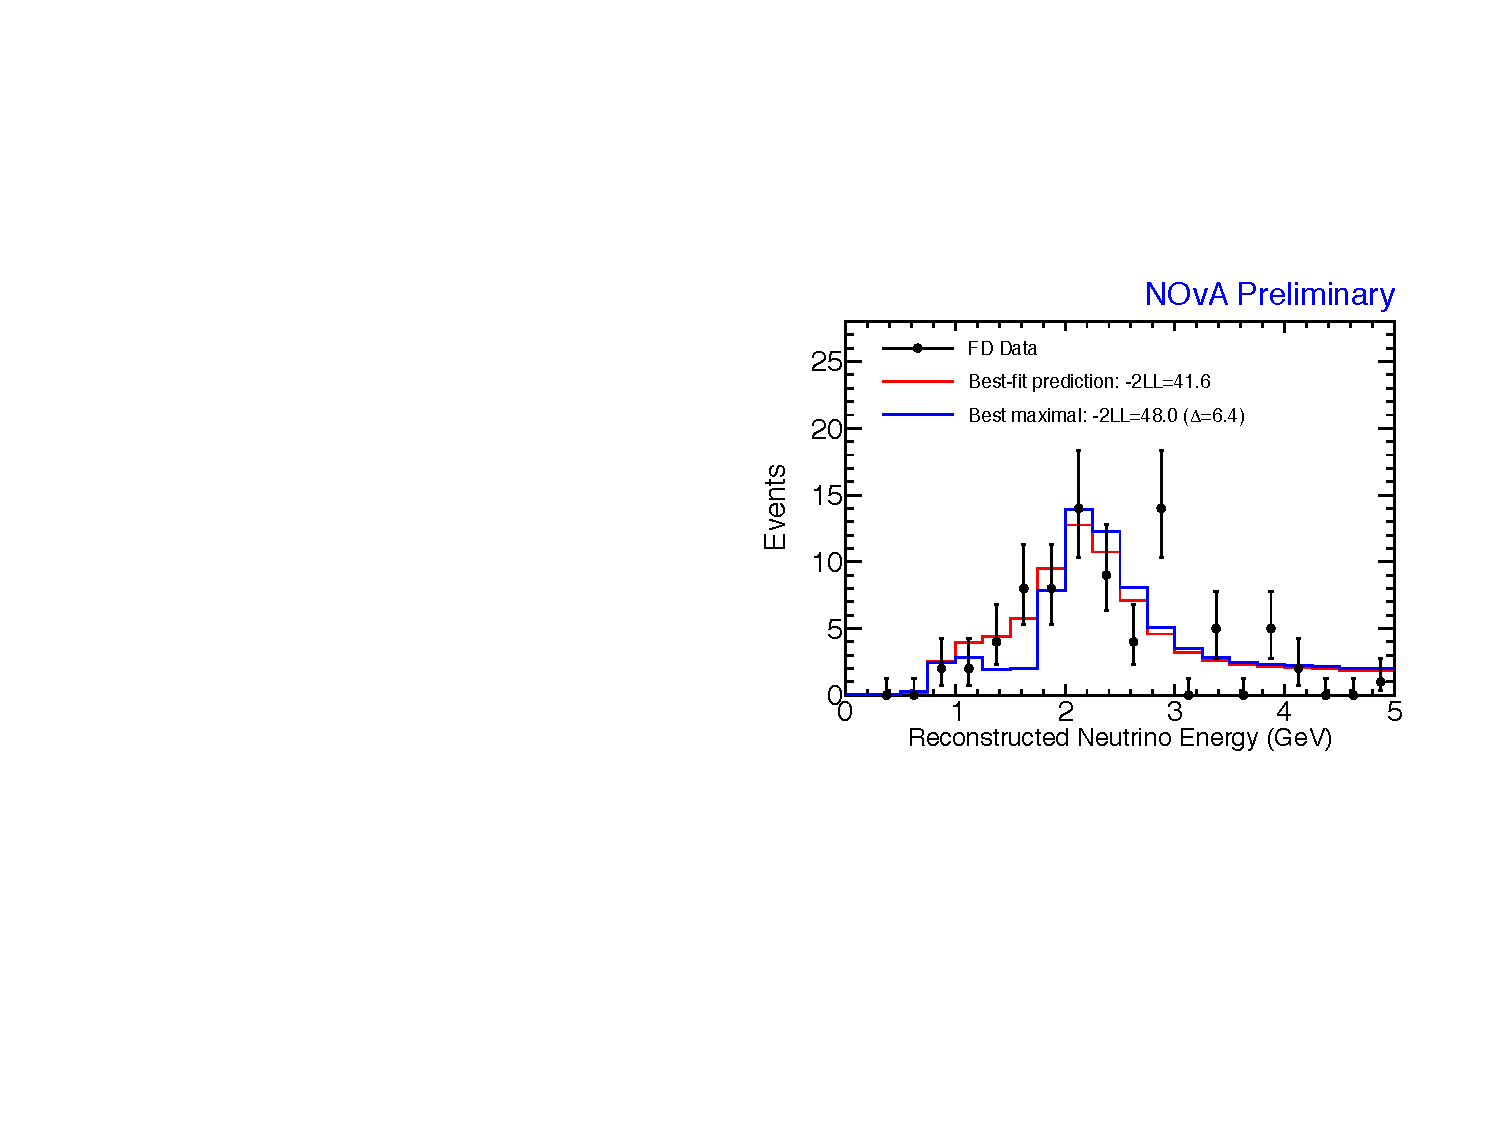
\includegraphics[width=0.6\linewidth]{figures/nova_comparison.pdf}
  \caption{Reconstructed energy spectrum in \nova for data, best fit and best fit assuming maximum mixing} \label{fig:atm-contour}
 \end{figure}

  \begin{figure}[htbp]
\centering
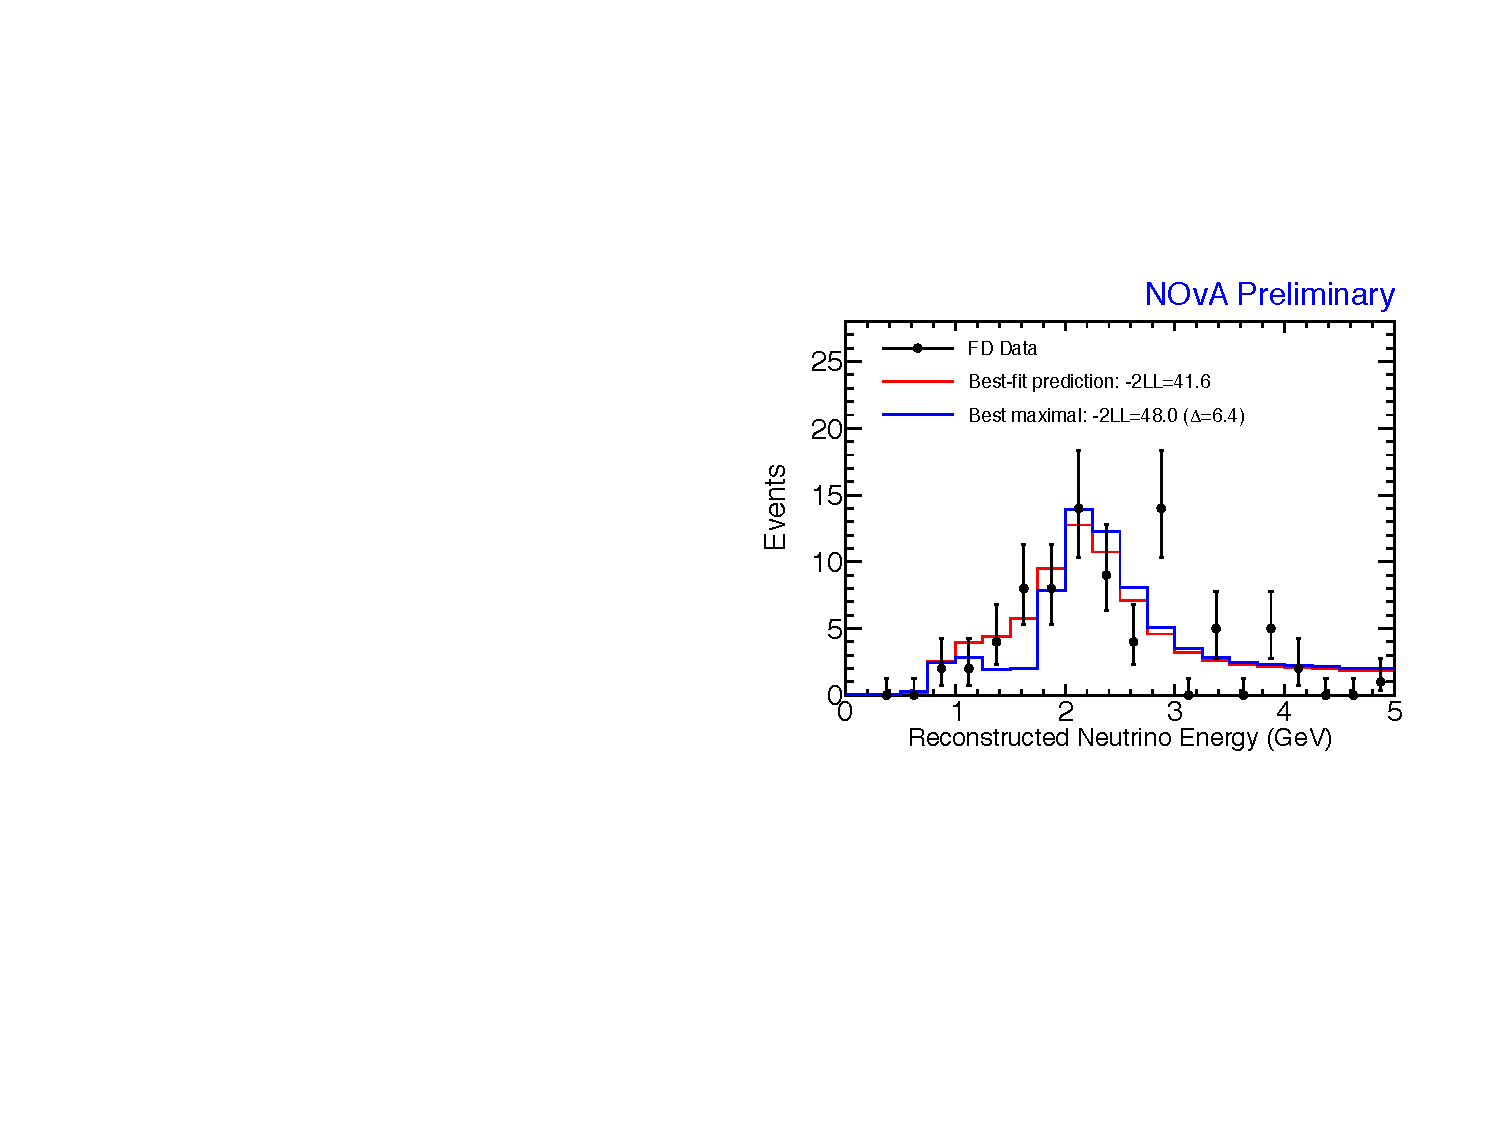
\includegraphics[width=0.6\linewidth]{figures/nova_comparison.pdf}
  \caption{Reconstructed energy spectrum in \nova for data, best fit and best fit assuming maximum mixing} \label{fig:atm-contour}
 \end{figure}

 
 
 
 \subsubsection{Evidence for $\nu_\tau$ appearance}

The OPERA experiment on the CERN to Gran Sasso neutrino beam, taking data between 2008 and 2012, was designed to test the $\nu_\mu \rightarrow \nu_\tau$ appearance hypothesis. The detector is based on the Emulsion Cloud Chamber technique, with 1800 ton of nuclear emulsion detectors in the forms of bricks, each brick being composed of a stack of nuclear emulsion film and lead plates. This target, capable of sub-micrometric track resolution, is devoted to the study of the neutrino interaction vertex and the particles associated to it. The identification of the $\tau$ leptons relies mainly on their characteristic kink (Fig.~\ref{fig:opera}) due to the decay $\tau \rightarrow h \nu_\tau$, or $\tau \rightarrow l \nu_\tau \bar \nu_l$, where $h$ is a charged meson, and $l$ is an electron or a muon. Another signature is related to the decay $\tau \rightarrow 3 h \nu_\tau$ where the short $\tau$ track ends in a three-pronged vertex. The target detectors are complemented by scintillator trackers and muon spectrometers. 

OPERA has observed 5 $\nu_\tau$ candidate events \cite{Agafonova:2015jxn} with a total background of 
$0.25 \pm 0.05$ events, mainly coming from decays of charmed particles. This corresponds to a 5.1 $\sigma$ observation of $\nu_\tau$ production in an oscillated $\nu_\mu$ beam. 

The Super-Kamiokande collaboration has also searched for $\nu_\tau$ appearance in multi-ring events to test the hypothesis of $\nu_\mu \rightarrow \nu_\tau$ oscillations~\cite{Abe:2012jj}. While the selected sample is affected by large backgrounds, there is an excess of tau-like events in the upward-going direction with a significance of 3.8 $\sigma$, offering a complementary confirmation of the OPERA result.  
 
\begin{figure}[htbp]
\centering
%\includegraphics[width=0.5\linewidth]{energy_miniboone.eps}
%\includegraphics[width=0.6\linewidth]{figures/topology_modified.pdf}
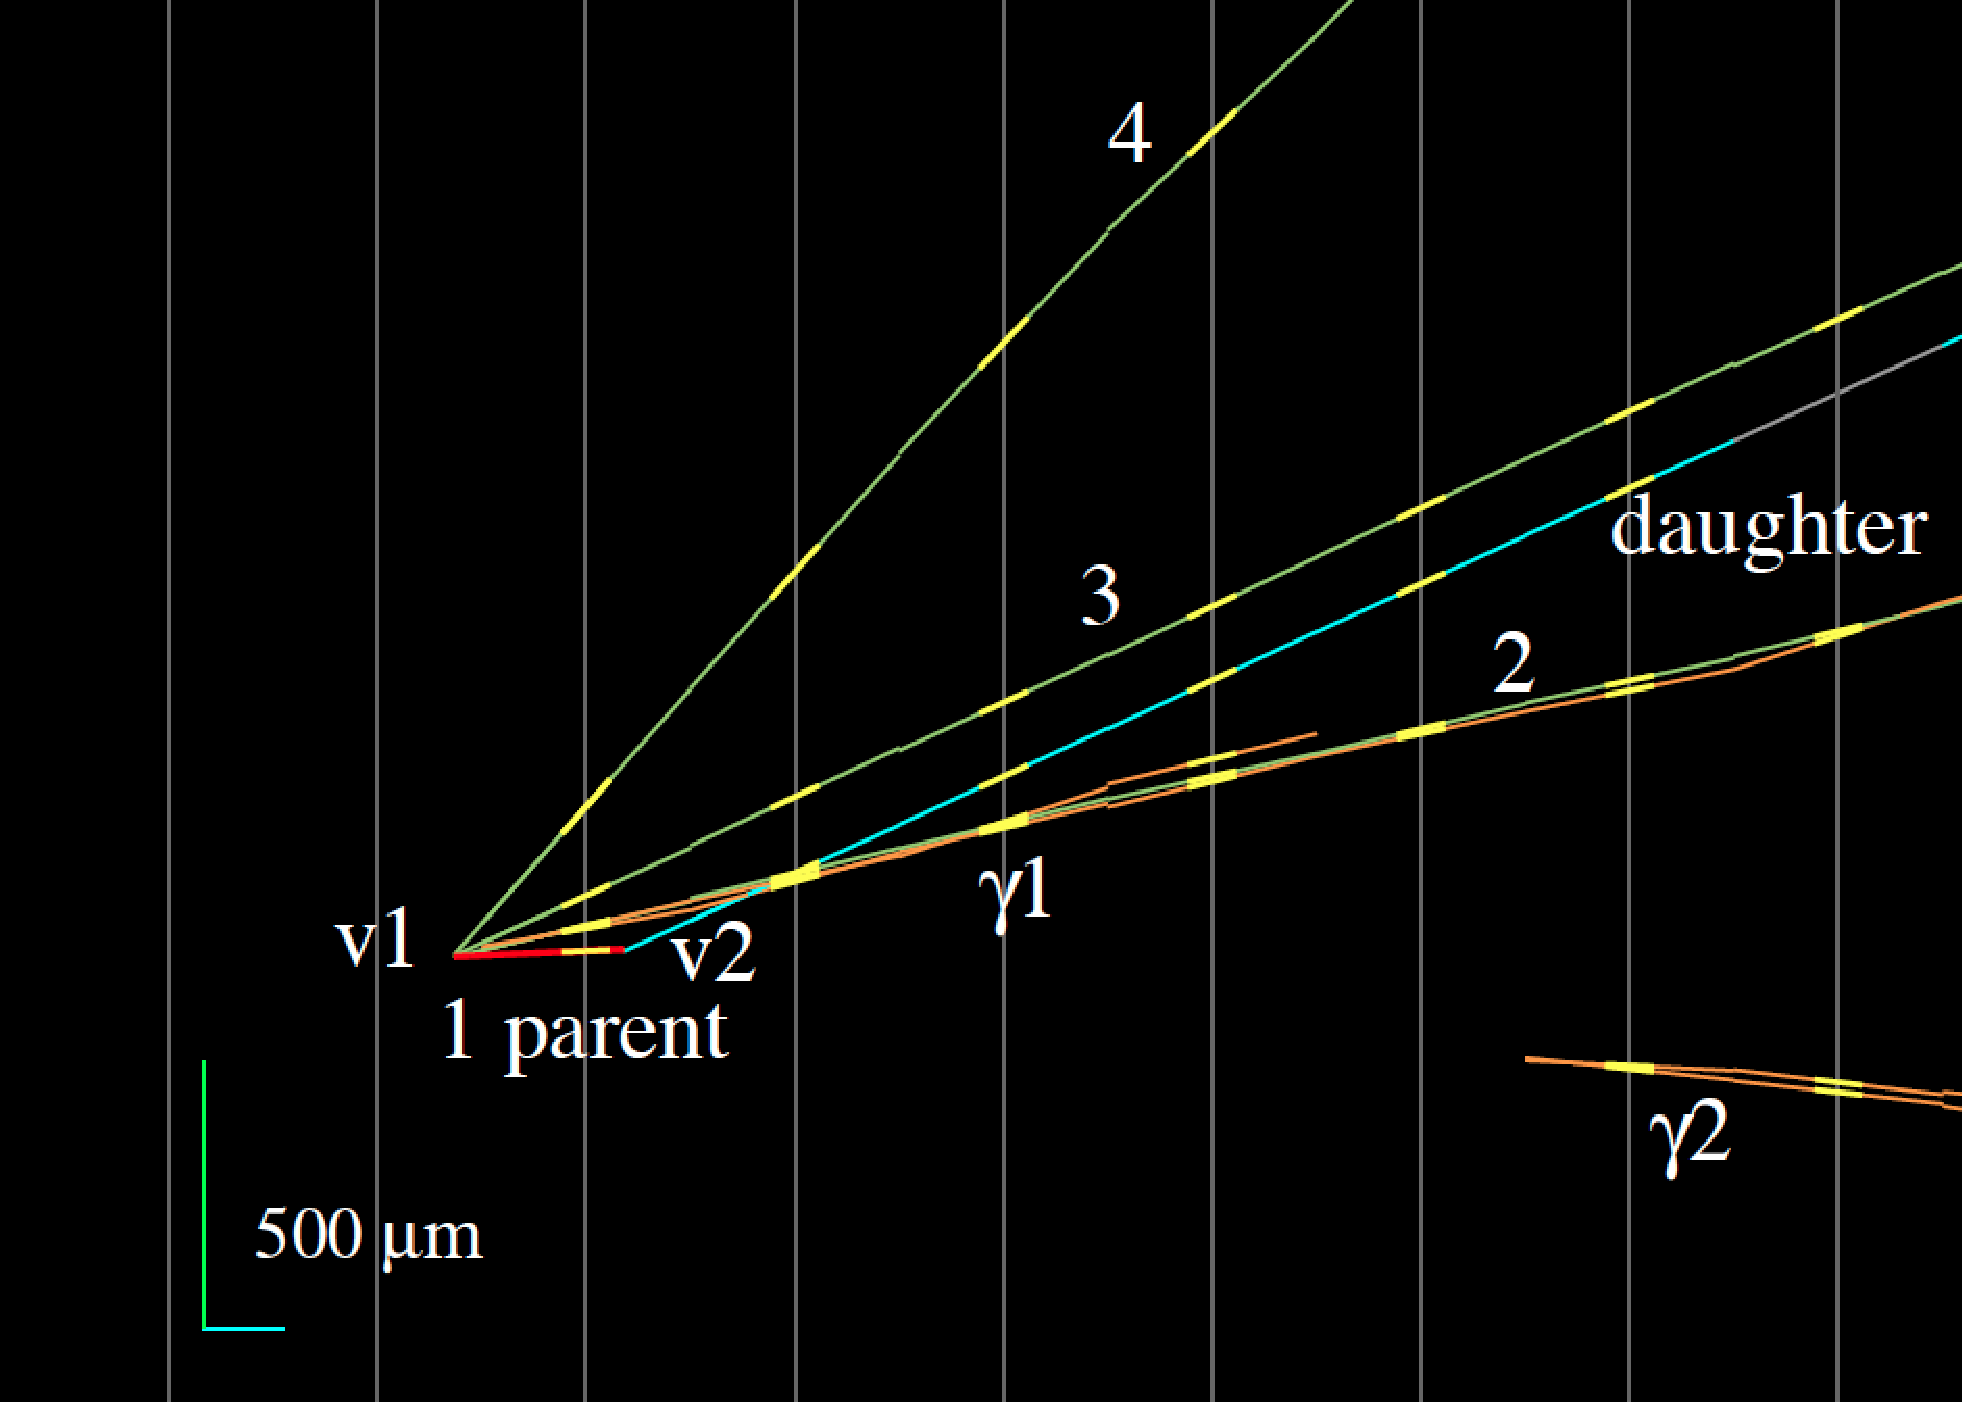
\includegraphics[width=0.6\linewidth]{figures/tau4.pdf}
  \caption{
Event display of the fourth $\nu_\tau$ candidate event from the OPERA 
experiment~\cite{DICRESCENZO2015186} in the
horizontal projection longitudinal to the neutrino direction.
The primary and secondary vertices are indicated as V$_0$ and
V$_1$ , respectively. The kink between the parent and daughter track, a feature of $\tau$ lepton decays, is clearly visible. The yellow stubs represent the track segments as measured in the emulsion films.  
}
 \label{fig:opera}
 \end{figure}

